\documentclass[l4proj.tex]{subfiles}
\begin{document}    

This chapter will look into the agile project management concepts that RViT is built upon and then examine the positive and negative aspects of three market-leading agile project management tools.

\section{Agile project management}
Agile methodology support is at the core of any project management tool designed for agile teams.

\subsection{Requirement Identification}
In agile project management, requirements identification is carried out throughout the life-cycle of the project. A just-in-time approach is typically used to convert the identified requirements into epics and user stories that can be prioritised by an agile team (\cite{Schon2017}). Good user story practises are essential to effective software development, templates can be used to aid teams in writing good user stories, while a definition of done can help developers understand what is required for a user story to be completed (\cite{Silva2017}).

Epic and user story mapping allows for developers to understand which story belongs to each epic. By being able to reorder these elements, developers can visually prioritise epics and user stories without having to use extremely fine-grained priority choices.

User stories can also contain a wealth of other information to help developers better understand their purpose. Category tagging can allow teams to identify what types of development a story might require, allowing for streamlined user assignment. Story points can allow teams to estimate how long user stories will take to complete, helping them to prioritise work effectively (\cite{Coelho2012}). 


\subsection{Visualising Progress with Kanban Boards}
Originally based on the lean manufacturing process used by Toyota, the applications of kanban boards are far reaching (\cite{Ahmad2018}). The main goal of a kanban board is to help a team visualise workflow. This process can often be helpful for agile project management.

A kanban board is based on a series of columns, as work progresses through these columns the workflow can be visualised and any bottlenecks or blockers can be easily identified. Work in progress limits can also be set on columns, forcing developers to work on a limited number of stories reducing their scope of attention.


\subsection{Visible Business Values}

Epics and user stories typically have business value associated with them. However the perceived value of an epic or user story tends to differ between stakeholders and developers (\cite{Gregory2020}). While user stories should aim to convey the value of a story using the INVEST criteria (\cite{Buglione2013}), these are often ambiguous. By defining a subset of business values, custom to a particular agile team, these can be used in epics and user stories to allow for a quick, streamlined value identification process for both stakeholders and developers. By making it easy for developers to identify business values it is also hoped that these will be taken into consideration during the prioritisation process and become a more integral part of an agile team's workflow. 

Highlighting the business value of an epic or user story will also help developers understand the purpose behind a particular task, hopefully increasing knowledge surrounding the utility cost of the task and increasing developer motivation (\cite{Wigfield2000}). 

\section{Existing Products}
There are many pre-existing agile project management tools on the market with considerable funding and industry backing. This selection provides a review of three industry leading tools, identifying the strengths and weaknesses of each and explaining were RViT finds its niche among these competitors.


\subsection{Jira}
Jira is a state-of-the-art project management tool, servicing over 65,000 companies across the globe (\cite{JiraUsers}). The tool offers extensive customisation options and supports a variety of agile methodologies including scrum and kanban, as seen in Figure (\ref{fig:Jira kanban}).
Jira also provides out-of-the-box metric reporting including burndown and velocity charts as well as cumulative flow diagrams (\cite{JiraReports}). Atlassian Open DevOps also automatically connects Jira with any of Atlassian's partner tools such as GitHub and BitBucket without the traditional overhead (\cite{JiraDevOps}). As an established tool, Jira also provides extensive documentation, not just on the application itself but also on agile methodologies themselves.

\begin{figure}[h!]
\begin{center}
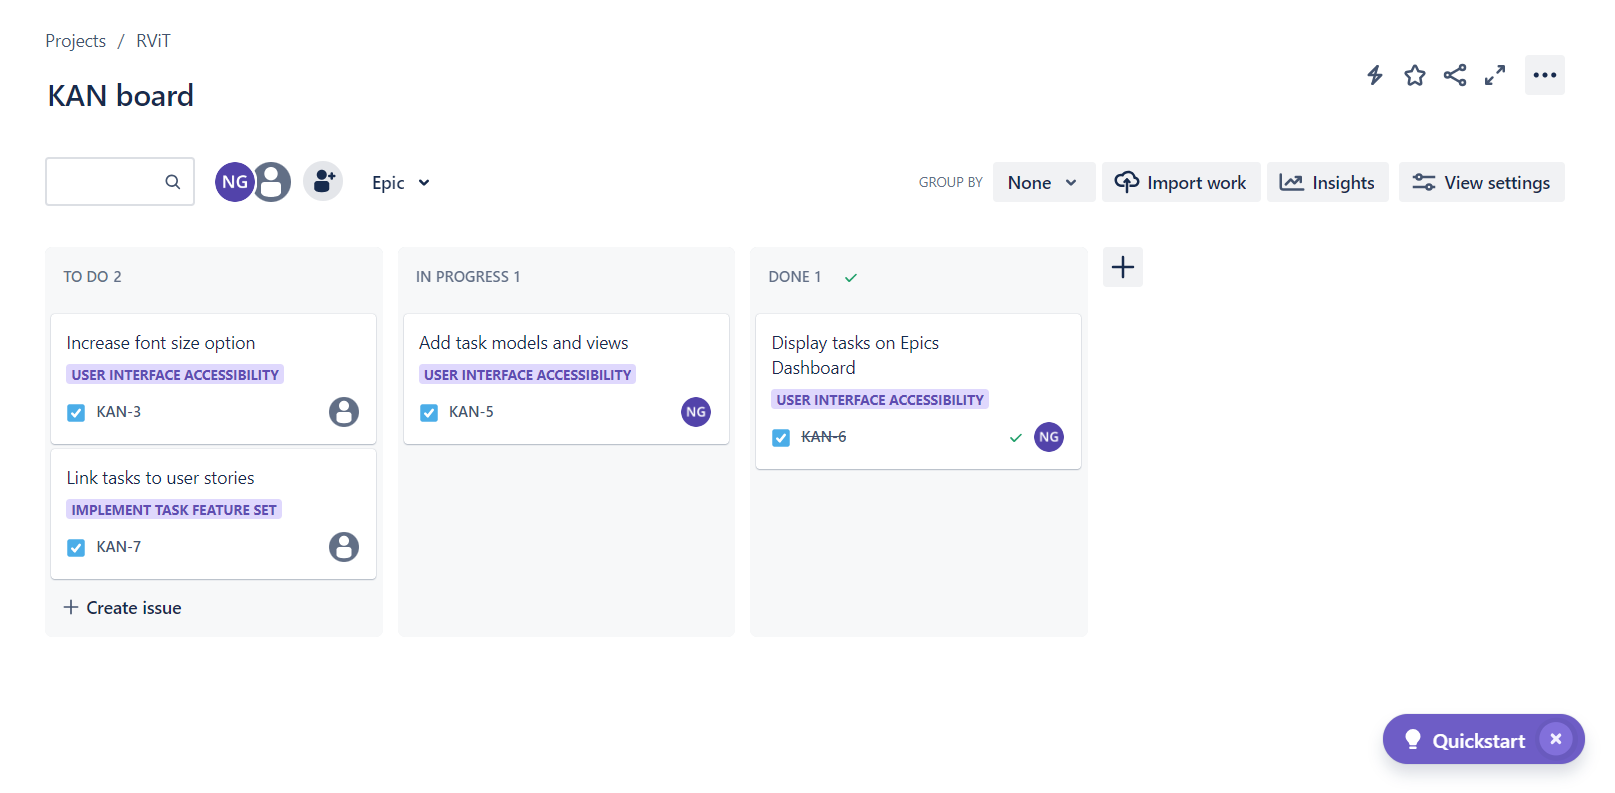
\includegraphics[scale=0.35]{dissertation/images/JiraKanbanBoard.png}
\caption{Example Jira kanban board}
\label{fig:Jira kanban} 
\end{center}
\end{figure}

As Jira is part of the Atlassian software set, the Atlassian Market place provides additional third-party Jira plug-ins and integrations to allow agile teams to further personalise their experience.  

One of the common criticisms of Jira is that the number of features it supports can be overwhelming for unfamiliar users and leads to a steep learning curve (\cite{JiraProblemsFeatures}). The amount of customisability can also be a problem with teams sometimes creating unintuitive dashboards with no real attention paid to the developer experience (\cite{JiraProblemsFlexible}). Jira is also only free to use for teams of up to 10 developers, with a slightly limited feature set. RViT aims to combat these issues by providing a free-to-use streamlined approach to kanban development that cuts out unnecessary overhead.


\subsection{Trello}
Trello is another Atlassian project management tool, though unlike Jira it has a significantly reduced feature set, focusing on kanban methodology support as seen in Figure \ref{fig:Trello kanban}. Another difference to Jira, is Trello is pitched as a general project management tool as opposed to an agile one. This means typical agile methodology support such as Epic creation is not present in Trello.

Similarly to Jira, Trello also has its own marketplace where you can add third party extensions called 'power-ups'. Power-ups can be anything from adding a priority component to a story to adding GitHub integration.

Trello is user friendly and intuitive to use with many example templates to quick-start a board. However, the free version only supports the kanban board itself and not any of the other views such as the dashboard or calendar view \cite{TrelloPricing}. RViT plans to create a similarly intuitive interface but with more out of the box agile methodology support such as allowing users to create epics, define definitions of done, and add clear tags, values and priorities.


\begin{figure}[h!]
\begin{center}
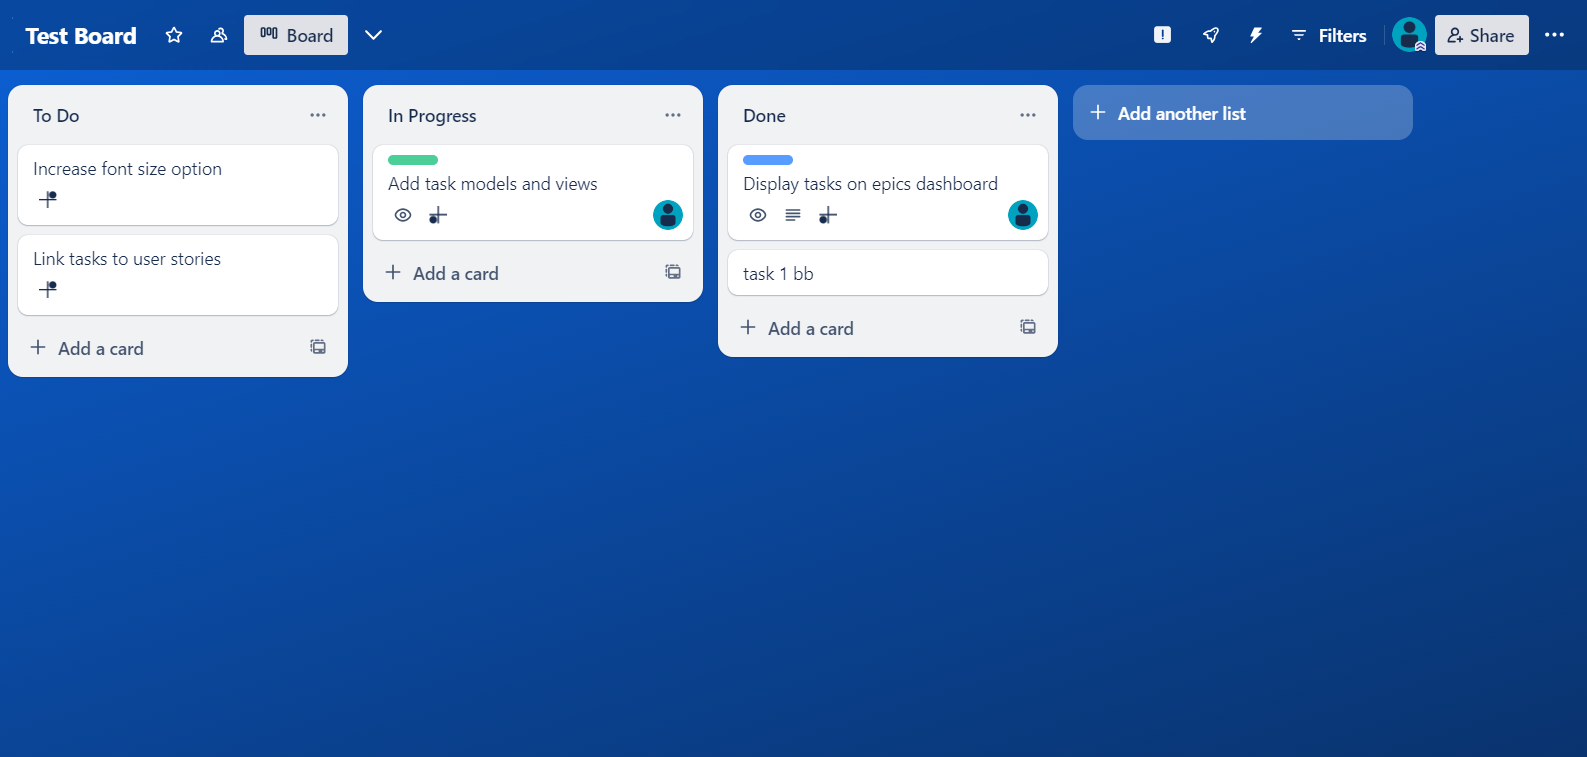
\includegraphics[scale=0.35]{dissertation/images/TrelloKanbanBoard.png}
\caption{Example Trello kanban board}
\label{fig:Trello kanban} 
\end{center}
\end{figure}

\subsection{GitHub Issues and Projects}
GitHub comes with built-in issue tracking support. Users can define issues and create custom issue templates to simplify the issue adding process. GitHub also allows developers to add customisable labels to a project and define milestones to add support for scrum-based teams. GitHub issues and projects are also accessible from the GitHub repository itself, meaning a secondary application does not have to be used. These tools are also completely free to use unlike Jira and Trello.


GitHub projects support three different views of a repository's issues, kanban board-based, table-based and roadmap-based. These views are intuitive to use but are not very visually appealing due to the lack of colour as seen in Figure \ref{fig:GitHub kanban}. As well as this, the information that a developer can gain without clicking into an issue is limited with there being no priority support and any labels the issue has not being visible until the issue is clicked into.

\begin{figure}[h!]
\begin{center}
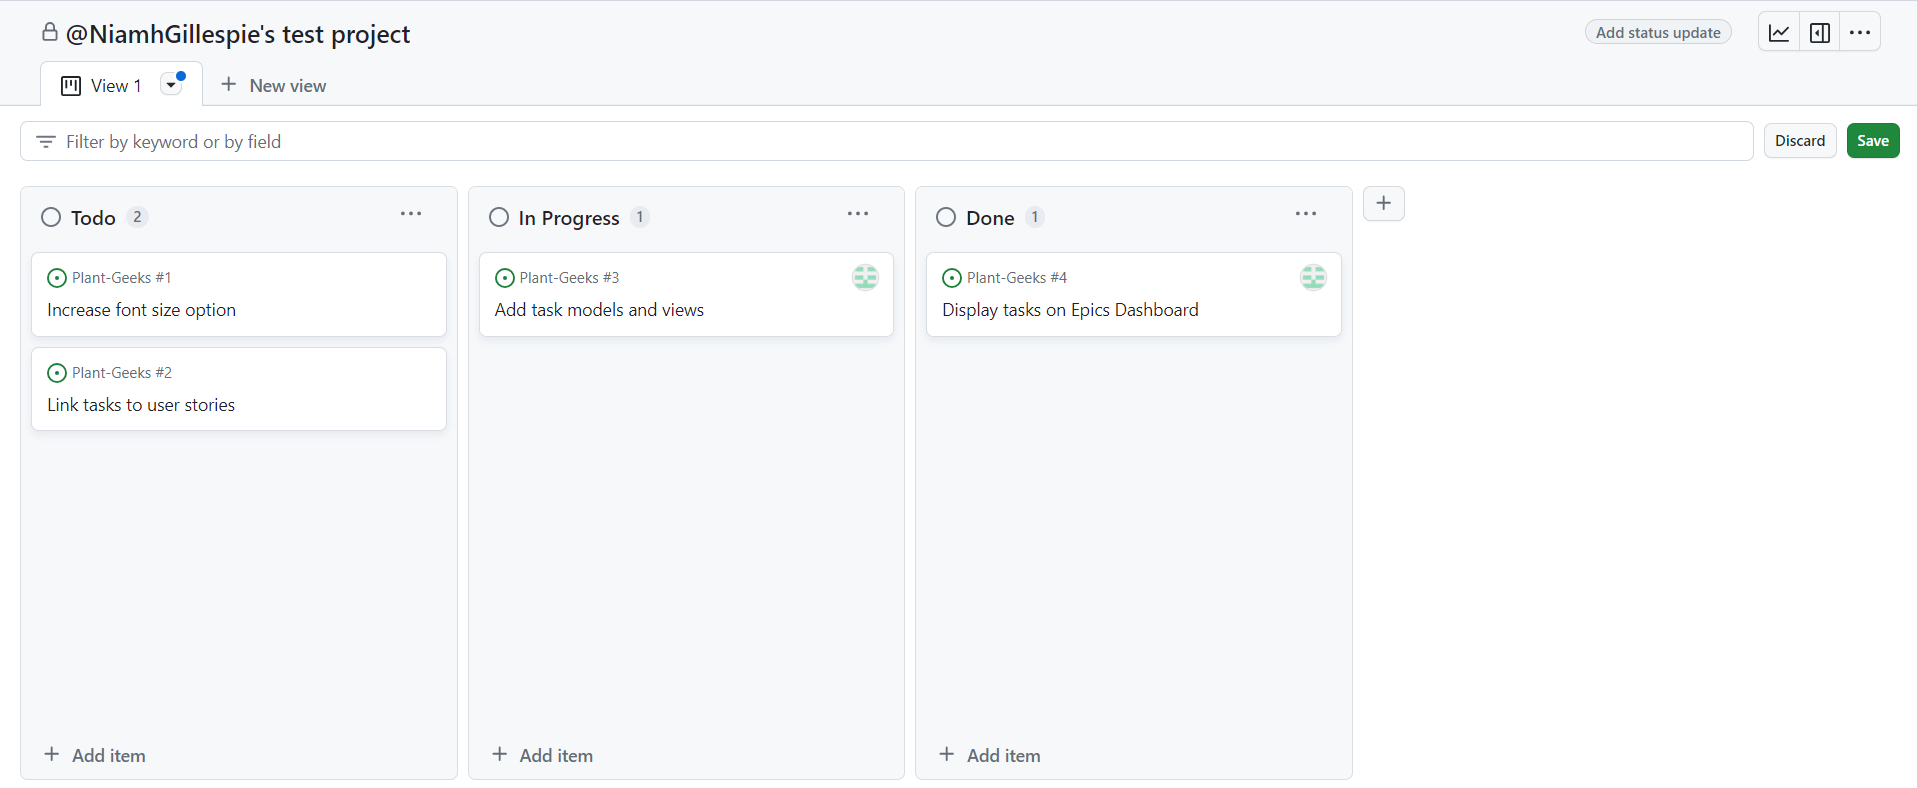
\includegraphics[scale=0.35]{dissertation/images/GitHubKanbanBoard.png}
\caption{Example GitHub kanban board}
\label{fig:GitHub kanban} 
\end{center}
\end{figure}


Like Trello, GitHub also lacks support for agile concepts like epics. RViT aims to support these concepts while also providing a more aesthetically pleasing user interface. 

\end{document}